\section{Cuestionario General}
En esta primera secci\'on se presentan las preguntas relacionadas con las generalidades de la empresa, que permiten obtener de primera mano informaci\'on sobre la direcci\'on, administraci\'on, productos y estructura de la empresa. M\'as adelante se indagar\'a sobre cada \'area en particular.

\subsection{Generalidades}

	\paragraph{Pregunta}
	 ?`Cu\'al es la antig\"{u}edad de la empresa en el pa\'is?  ?`Y la del grupo Marsans?
	\paragraph{Respuesta}
	En el pa\'is Marsans tiene 40 a\~{n}os. En el mundo 101 a\~{n}os.

	\paragraph{Pregunta}
	 ?`De qu\'e forma se despliega geogr\'aficamente?  ?`Cu\'ales son sus sedes, filiales, puntos de venta?  ?`Est\'a presente en todo el pa\'is?
	\paragraph{Respuesta}
	Tiene su casa central en Capital Federal y sucursales en Rosario y C\'ordoba. Tambi\'en representaciones en Mar del Plata, Santa Fe y Neuqu\'en.

	\paragraph{Pregunta}
	 ?`En qu\'e rama de la industria se ubica?  ?`Cu\'al es su participaci\'on en el mercado?  ?`Qu\'e empresas representan la competencia?
	\paragraph{Respuesta}
	Marsans es un operador mayorista de turismo. Es uno de los l\'ideres a nivel nacional e internacional en operaci\'on mayorista. La competencia est\'a conformada por Julia, Eurovips, Eurotour, Piamonte, entre otros.

\subsection{Organigrama}
	A continuaci\'on se presenta el organigrama completo de la empresa, y se lo clasifica seg\'un los conceptos vistos en clase.

	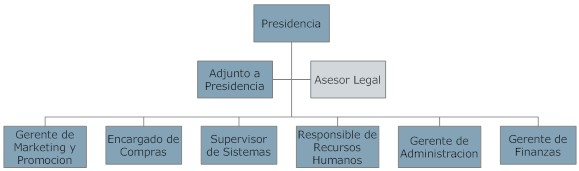
\includegraphics[scale=0.45]{Images/organigrama-marsans.png}

	\paragraph{Pregunta}
	 ?`Qu\'e cantidad de personal hay en el nivel dirigencial?  ?`En el operativo?  ?`En el de supervisi\'on? PRESENTAR UNA DISTRIBUCION PORCENTUAL
	\paragraph{Respuesta}
	A nivel Dirigencial, hay 3 personas. En la parte operativa 46. En el de supervision 8.

	\paragraph{Pregunta}
	 ?`Qu\'e cantidad de personal es efectivo, y cu\'al contratado? CALCULAR RELACION
	\paragraph{Respuesta}
	Todo el personal de la compa��a es efectivo.

	\paragraph{Pregunta}
	 ?`C\'omo afectan las fluctuaciones de la actividad a la incorporaci\'on o desvinculaci\'on de personal?
	\paragraph{Respuesta}
	El personal suele mantenerse estable para las temporadas altas y bajas, s\'olo que en las altas suele contratarse personal de refuerzo, debido a la mayor demanda de productos.

\subsection{Direcci\'on}

	\paragraph{Pregunta}
	 ?`Cu\'al es el objetivo general de la empresa?
	\paragraph{Respuesta}
	El objetivo de la empresa es continuar siendo una multidestino (se comercializan todo tipo de destinos) y rentabilizar cada vez m�s cada venta.

	\paragraph{Pregunta}
	 ?`Cu\'ales son los pilares de la estrategia corporativa?
	\paragraph{Respuesta}
	Brindar un excelente servicio y calidad en la atenci\'on, para diferenciarnos de la competencia.

	\paragraph{Pregunta}
	 ?`Ha atravesado la empresa un proceso de dise\~{n}o organizacional formal?  ?`Es actualizado mediante cambios organizacionales? Caso positivo,  ?`qu\'e tan frecuentemente?
	\paragraph{Respuesta}
	Se ha realizado una restructuraci\'on del sector nacional, luego de la salida de Marsans del gerenciamiento de Aerol�neas Argentinas. Esto ha hecho que algunas unidades de negocio se fusionen con otras.

	\paragraph{Pregunta}
	 ?`Cu\'ales son los mecanismos de toma de decisi\'on y determinaci\'on de estrategias utilizados?
	\paragraph{Respuesta}
	Las tomas de decisi\'on a nivel institucional, pasan por presidencia, con el consenso previo de los accionistas en Madrid. Las operativas son realizadas por cada gerente o supervisor de departamento.

	\paragraph{Pregunta}
	 ?`Cu\'al es el grado de participaci\'on en las decisiones de los distintos niveles jer\'arquicos? DETALLAR DECISIONES TOMADAS EN CADA NIVEL
	\paragraph{Respuesta}
	Todo el nivel de supervisi\'on y general tiene la misma injerencia en la toma de decisiones.

\subsection{Producci\'on}

	\paragraph{Pregunta}
	 ?`Qu\'e productos o servicios ofrece la empresa al mercado?
	\paragraph{Respuesta}
	Marsans es un multiproducto, ofrece paquetes tur\'isticos nacionales e internacionales a agencias minoristas de turismo, as\'i como tambi�n ofrece servicios receptivos para pasajeros extranjeros.

	\paragraph{Pregunta}
	 ?`Alcanzan estos productos el \'exito perseguido?
	\paragraph{Respuesta}
	Si, aunque la crisis local y mundial, hizo que haya disminuido la cantidad de pasajeros. Viajar es un lujo y es uno de los aspectos que los argentinos recortan cuando hay crisis. No han tenido el mismo resultado los paquetes corporativos, que siguen manteniendo su nivel.

	\paragraph{Pregunta}
	 ?`Planea ofrecer en el corto plazo nuevos productos o servicios?
	\paragraph{Respuesta}
	No, por ahora los que manejamos cada temporada.

	\paragraph{Pregunta}
	 ?`Se discontinuaron en el \'ultimo tiempo productos o servicios? ?`Por qu\'e?
	\paragraph{Respuesta}
	No, por ahora seguimos ofreciendo los mismos, aunque con menos pasajeros.

	\paragraph{Pregunta}
	 ?`Se terceriza alguna parte del proceso de producci\'on?  ?`Por qu\'e? (disminuir costos, abastecer la demanda sin aumentar el tama\~{n}o de la empresa, etc.)
	\paragraph{Respuesta}
	Se terceriza la limpieza, seguridad  y la mensajer�a. 

\subsection{Recursos Humanos}
	\paragraph{Pregunta}
	 ?`Cu\'antas personas est\'an destinadas a este \'area?  ?`Qu\'e proporci\'on representa del total de la empresa?
	\paragraph{Respuesta}
	Hay una sola persona en el departamento de RRHH que es la responsable del mismo.

	\paragraph{Pregunta}
	 ?`Est\'an especificamente capacitados en el \'area de RR.HH.?
	\paragraph{Respuesta}
	S�, la responsable es Psic\'olaga y cuenta con un posgrado en Organizaci\'on y Conducci\'on de RRHH, dictado por la facultad de Psicolog�a de la UBA.

	\paragraph{Pregunta}
	 ?`Qui\'en pide (o est\'a autorizado a pedir) la incorporaci\'on de personal?  ?`Qui\'en decide cu\'ando reclutar nuevo personal?
	\paragraph{Respuesta}
	La incorporaci�n de personal debe ser autorizada por el Director, �l define cu\'ando y c\'omo.
	
	\paragraph{Pregunta}
	 ?`Cu\'ales son los m\'etodos usuales de reclutamiento de personal?  ?`Involucran personal de otras \'areas?
	\paragraph{Respuesta}
	Se recluta personal a trav\'es de avisos en los medios del Trade, a trav\'es de paginas web especializadas (Bumeran, Computrabajo) y en algunos casos a trav�s de consultoras.
	
	\paragraph{Pregunta}
	 ?`Hay pol\'iticas de bono?  ?`Cu\'ales?
	\paragraph{Respuesta}
	Existe un plus que se abona a las unidades de negocio que alcazaron mensualmente los objetivos del \'area. Se llama PRV y consiste en el 8,33\% del salario b\'asico.
	
	\paragraph{Pregunta}
	 ?`Hay plan de carrera?  ?`Incluye a todo el personal?
	\paragraph{Respuesta}
	En este momento se est� desarrollando.
	
	\paragraph{Pregunta}
	 ?`Se capacita al personal?  ?`Dentro o fuera de la empresa?  ?`Qui\'en se encarga de hacerlo?
	\paragraph{Respuesta}
	Las capacitaciones se realizan \textit{in company} y fuera de la empresa. Se contratan consultoras para realizar las mismas, los proveedores suelen tambien capacitar al personal. 